\documentclass{ximera}
%% handout
%% nohints
%% space
%% newpage
%% numbers

%% You can put user macros here
%% However, you cannot make new environments

\graphicspath{{./}{firstExample/}{secondExample/}}

\usepackage{url}
\usepackage{tikz}
\usepackage{tkz-euclide}
\usetkzobj{all}


\tikzstyle geometryDiagrams=[ultra thick,color=blue!50!black]
\pgfplotsset{compat=1.8}
  \usepackage[T1]{fontenc}
  \usepackage[utf8x]{inputenc} %% we can turn off input when making a master document

\prerequisites{none}


\title{Taxes}

\begin{document}
\begin{abstract}
We perform calculations involving a variety of tax types.
\end{abstract}
\maketitle
\begin{quote}
Our new Constitution is now established, and has an appearance that promises permanency; but in this world nothing can be said to be certain, except death and taxes. --- Benjamin Franklin, $1789$
\end{quote}

Taxes, in some form or another, are familiar to all of us. Local, state, and federal government agencies all levy taxes of various types and most have taken pains to ensure that collection of taxes is automatic, meaning that the calculations involved in taxation are often hidden from view.

Some taxes are simple percentage rates, such as most sales taxes. The $2014$ sales tax rate in Henderson, Nevada is $8.1\%$, meaning that for every $\$100$ in taxable purchases an additional $\$8.10$ is collected in tax.

Other taxes, like income tax, combine percentage calculations with more complicated delineations of income into brackets. For example, in $2014$ a single taxpayer with $\$18,000$ in taxable income will be charged a federal tax rate of $10\%$ An equivalent filer with $\$125,000$ in taxable income will owe slightly over $18\%$. (\href{http://www.forbes.com/sites/kellyphillipserb/2013/10/31/irs-announces-2014-tax-brackets-standard-deduction-amounts-and-more/}{Forbes article})

Still other taxes involve more complicated computations involving a wide variety of factors. 

A \emph{subsidy} can be thought of as a negative tax --- money is paid from the government to an entity for a particular economic, social, or political purpose. For example, during the Great Depression food prices dropped considerably because farms produced more crops than the market demanded. The low food prices meant farmers couldn't make enough selling their crops to pay their bills and a large number of farmers defaulted on their farm (and home) loans. To counteract this situation, Congress passed the Agriculture Adjustment Act in 1933. This legislation offered farmers money for \emph{not} growing certain crops. This money offset the farmers' debt and reduced the quantity of those crops, leading to an increase in food prices that further benefited farming communities.

The practice of offering subsidies, including for agriculture, continues in large measure today despite substantial controversy surrounding the practice.

A \emph{tariff} is a type of tax that is levied on goods produced in one location and sold in another location, such as goods imported from another country. Tariffs are sometimes imposed so that goods manufactured cheaply in another part of the world cost the same as or more than goods produced near where they are sold. This is done so that the more expensively produced goods are not undersold by cheaper goods from foreign competitors.

\begin{question}
Watch the video at \href{http://www.showme.com/sh/?h=jUoQ4fo}{http://www.showme.com/sh/?h=jUoQ4fo} to see an example of using a model of consumer behavior similar to that used in the following problem about tariffs.

Suppose that when consumers are faced with purchasing either of two light-bulbs that differ in price by $\$d$, the proportion of them that will buy the cheaper light-bulb is $\displaystyle \frac{1}{1+2^{-4d}}$. A graph of this function is shown below.
\begin{image}
%\begin{tikzpicture}[>=stealth,scale=1.5,samples=200,smooth]
%\begin{axis}
%[xlabel={Difference between products' prices},ylabel={\% that buy cheaper product},xmin=0,xmax=1,ymin=0,ymax=1,xtick={0,0.25,0.5,0.75,1},xticklabels={0\cent,25\cent,50\cent,75\cent,\$1.00},ytick={0,0.2,0.4,0.6,0.8,1},yticklabels={0\%,20\%,40\%,60\%,80\%,100\%},grid=major]
%\addplot[color=blue,ultra thick]{1/(1+2^(-4*x))};
%\addplot[fill=red,nodes near coords=\emph{(50\cent, 80\%)},every node near coord/.style={anchor=335}] (0.5,0.8) circle (0.015);
%\end{axis}
%\end{tikzpicture}
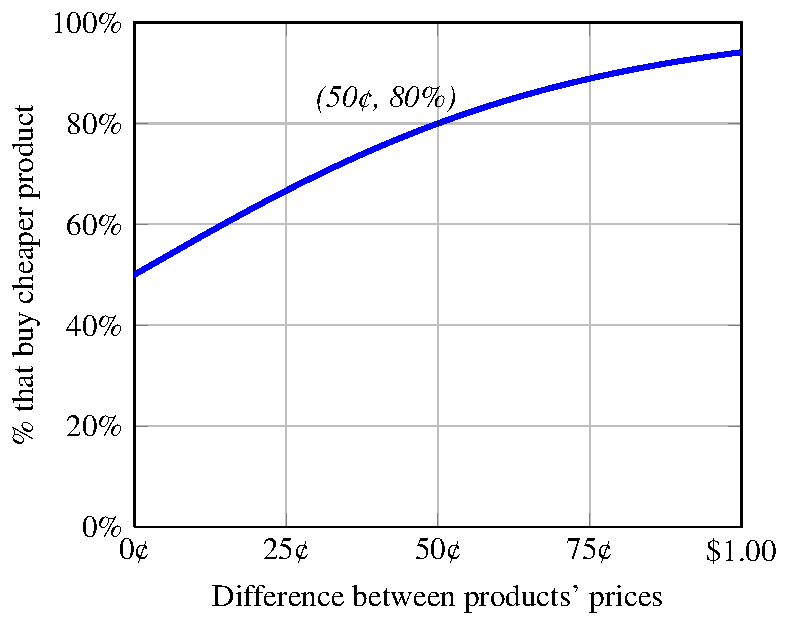
\includegraphics{buyingproducts.pdf}
\end{image}
For example, if one light-bulb is $\$0.50$ more than the other, then $\dfrac{1}{1+2^{-4\times 0.50}}=0.8=80\%$ of consumers will purchase the cheaper light-bulb.

Suppose consumers in coastal California buy $1,500,000$ light-bulbs in a given month and one of them is $\$0.10$ more expensive than the other. Approximately how many of the cheaper light-bulbs will be bought?


 \begin{multipleChoice}
    	\choice[correct]{$850$ thousand}
        \choice{$750$ thousand}
        \choice{$700$ thousand}
        \choice{$1$ million}
        \choice{$500$ thousand}
    \end{multipleChoice}
\begin{hint}
Evaluate $\dfrac{1}{1+2^{-4\times 0.10}}$.
\end{hint}
\begin{hint}
How many light-bulbs, out of $1,500,000$ does $\dfrac{1}{1+2^{-4\times 0.10}}$ represent?
\end{hint}

\end{question}

\begin{question}

Tom operates a light-bulb factory in coastal California. Javier operates a similar factory in rural Nevada, where the costs of business are lower than in coastal California. If Tom's light-bulbs are $\$0.15$ more than Javier's, what proportion of consumers would purchase Javier's light-bulbs instead of Tom's? (Assume that Tom's and Javier's light-bulbs are the only light-bulbs for sale.)

\begin{multipleChoice}
\choice[correct]{About $60\%$}
\choice{About $40\%$}
\choice{About $85\%$}
\choice{About $15\%$}
\choice{About $50\%$}
\end{multipleChoice}
\begin{hint}
Use $\dfrac{1}{1+2^{-4d}}$ with $d=0.15$.
\end{hint}

\end{question}


\begin{question}
Suppose Tom must sell $\$1,000,000$ worth of light-bulbs in coastal California each month to break even.\footnote{Breaking even refers to having revenues exactly equal costs, so that although there are no losses, there is no profit either.} If Tom's light-bulbs sell for $\$1$ each while Javier's sell for $\$0.85$ each, what will be the effect of the $\$0.15$ price difference on Tom's business? Assume that consumers buy $1,500,000$ light-bulbs per month. 


\begin{multipleChoice}
    	\choice{Tom will make a large profit (over $\$100,000$/month)}
        \choice{Tom will make a small profit (under $\$100,000$/month)}
        \choice{Tom will break even}
        \choice{Tom will suffer a small loss (less than $\$100,000$/month)}
        \choice[correct]{Tom will suffer a large loss (more than $\$100,000$/month)}
    \end{multipleChoice}
\begin{hint}
$\dfrac{1}{1+2^{-4\times 0.15}}$ represents the proportion of consumers who will buy \emph{Javier's} light-bulbs. What proportion of consumers will buy \emph{Tom's} light-bulbs?
\end{hint}
\begin{hint}
How much money will the sale of those light-bulbs bring in for Tom's factory?
\end{hint}
\begin{hint}
How close is that amount of money to what Tom needs to break even?
\end{hint}

Nice work!
\end{question}

\begin{question}
In response to Javier's cheap light-bulbs, authorities in coastal California put a tariff of $\$0.45$ each on light-bulbs imported from Javier's factory. If customers buy $1,500,000$ light-bulbs per month, what will be the outcome of the tariff on Tom's business?


\begin{multipleChoice}
    	\choice{Tom will make a large profit (over $\$100,000$/month)}
        \choice[correct]{Tom will make a small profit (under $\$100,000$/month)}
        \choice{Tom will break even}
        \choice{Tom will suffer a small loss (less than $\$100,000$/month)}
        \choice{Tom will suffer a large loss (more than $\$100,000$/month)}
    \end{multipleChoice}
\begin{hint}
What will the total price of Javier's imported light-bulbs be, including his $\$0.85$ price and the tariff?
\end{hint}
\begin{hint}
Using the price of the light-bulbs, find $d$, the difference between the prices, and then use $\dfrac{1}{1+2^{-4d}}$ to find out what proportion of the consumers will buy Tom's now cheaper light-bulbs.
\end{hint}
\begin{hint}
How many of Tom's light-bulbs will consumers purchase at the price of $\$1.00$ each?
\end{hint}

Nice work!
\end{question}

\end{document}
